\documentclass{report}

\usepackage[english]{babel}
\usepackage{graphicx}
\usepackage[toc,page]{appendix}
\usepackage[colorlinks = true]{hyperref}

\graphicspath{ {./img/} }

\title{Requirements}
\author{Oscar de Leeuw}

\begin{document}
\maketitle
\tableofcontents
\newpage

\chapter{Requirements}
\newpage
\section{Game Rules}
These are the requirements of the game that the system should simulate.
\\ \\
Rules concerning game start and end.
\begin{center}
    \begin{tabular}{ | l | p{5.8cm} | p{4cm} |}
    \hline
    ID & Requirement & Remark \\ \hline
    GR01 & The board the game is played upon must be 8x8 big with 
    alternating color squares. &  \\ \hline
    GR02 & A game must always start with both players in the same position. 
    & See \hyperref[fig:Board_start]{\ref*{fig:Board_start}} for the defined
    position.\\ \hline
    GR03 & The game must always end in either a draw or 
    one player winning & \\ \hline
    GR04 & If a player cannot make a move without violating XXX and he is in 
    check, the game ends with that player losing. & 
    Win/Lose condition. Definition of 
    \hyperref[def:In_check]{in check}. \\ \hline
    GR05 & A player may resign at any point, 
    resulting in a win for the opponent. & Win/Lose condition.\\ \hline
    GR06 & If there is insufficient material to force a checkmate the game is
    a draw by default.
    & Draw condition. Insufficient material is defined
    \hyperref[def:Insufficient_material]{here}  \\ \hline
    GR07 & If one player can't make a move without violating XXX but he is not
    in check, the game ends in a draw.
    & Draw condition. Definition of 
    \hyperref[def:In_check]{in check}.  \\ \hline
    GR08 & If both players agree to draw the game must end in a draw.
    & Draw condition. \\ \hline
    GR09 & If there have been fifty moves, by each player, without a capture 
    or pawn move the game must end in a draw. & Draw condition. \\ \hline
    GR10 & If the same board position has occurred three times 
    the game must end in a draw. & Draw condition. Detailed definition of the 
    \hyperref[def:Threefold_repetition]{threefold repetition} \\ \hline
	GR11 & A game played under time control will end as a loss for a player who 				uses up all of their allotted time.
    & Win/Lose condition. Rule does not apply when the opponent is incapable of 				checkmating  \\ \hline


    \end{tabular}
\end{center}

%GR03 & A move by a player may never enable the opponent    to hit one's king. & M & \\ \hline

\begin{appendices}
\chapter{Figures}
\listoffigures

\begin{figure}[p]
    \centering   
    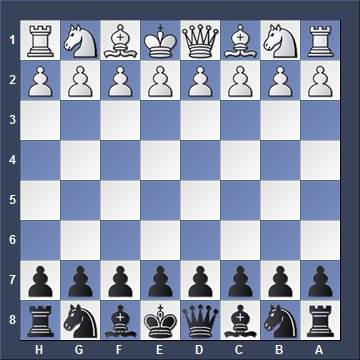
\includegraphics[scale=1]{Board_start.jpg}
	\caption[Game start]{The state of the board at the start of a game.}
    \label{fig:Board_start}
\end{figure}

\chapter{Definitions}

\subsection*{In check}
\label{def:In_check}
If player A is in a position such that on his next turn he could capture player B's king then player B is in check.

\subsection*{Insufficient material}
\label{def:Insufficient_material}
Insufficient material is defined as follows:
\begin{itemize}
    \item King against king;
    \item King against king and knight;
    \item King against king and bishop;
    \item King and bishop against king and bishop, when both bishops are on same
    coloured squares;
\end{itemize}

\subsection*{Threefold repetition}
\label{def:Threefold_repetition}
Threefold repetition occurs if the same player was to move three times in a row    and all pieces having the same rights to move, including the right to castle or capture en passant.
\end{appendices}

\end{document}

